% labels:
% cap:introducao
% sec:motivacao_proposta
% sec:tools
% sec:asteroids
% sec:gymretro
% sec:tensorflow
% sec:proposta

%% ---------------------------------------------------------------------------- %
\chapter{Introdução}
\label{cap:introducao}
%% ---------------------------------------------------------------------------- %

%Inteligência artificial, ou IA, é uma área de estudos que pode ser definida de diversas formas, como construir uma máquina que realize com sucesso tarefas tradicionalmente feitas por humanos, ou que aja como um humano.
%Diversas ciências mostraram-se importantes ao longo de sua história, como filosofia, matemática, computação e linguística, permitindo que profissionais de formações distintas pudessem contribuir para seus avanços.

Um tipo muito conhecido de inteligência artificial, ou IA, dos dias atuais é o que controla oponentes em jogos eletrônicos.
Na maior parte dos casos, elas seguem um conjunto pré-determinado de regras escritas pelo desenvolvedor com o intuito de criar um desafio para o jogador.
Entretanto, por mais que seja possível fazer a IA ter capacidades muito acima de seres humanos para jogar, elas não possuem a capacidade de se adaptar ao como seres humanos fazem para melhorar seu desempenho.
Quando pessoas não recebem ajuda externa ou leem um manual, normalmente elas aprendem e se adaptam por tentativa e erro, descobrindo o que as ações fazem e suas respectivas consequências.
Ao invés de explicitar as regras que a máquina deve seguir, é possível deixá-la aprender as que considerar melhor de maneira semelhante a humanos por meio de \textbf{aprendizado por reforço}, ou seja, por meio de tentativa e erro.

%É interessante a forma como seres humanos aprendem, em particular crianças pequenas e bebês.
%Eles fazem isso principalmente interagindo com o ambiente, tocando em objetos, tentando entender aquilo que os rodeia e qual o resultado de suas ações, mesmo que inconscientemente.
%Avanços em inteligência artificial nas últimas décadas permitiram que máquinas simulassem esse tipo de aprendizado por meio de \textbf{aprendizado por reforço}.

Entretanto, para muitos casos, somente esse tipo de técnica não é o suficiente.
Uma pessoa consegue inferir o que é inimigo e o que é terreno quando aparece na tela em poucos movimentos ou a partir de experiências passadas com jogos diferentes.
%Utilizando jogos como exemplo, uma pessoa consegue inferir o que é inimigo e o que é terreno quando aparece na tela do jogo em poucos movimentos ou até já supor a partir de experiências passadas com jogos diferentes.
Para um computador, um pixel que mude de posição já faz ele não conseguir mais distinguir o que está vendo, tendo que reaprender a cada nova combinação de pixels detectada.
Em outras palavras, seres humanos conseguem abstrair as informações que enxergam com facilidade, enquanto computadores não.
Se IAs não conseguem mais identificar um objeto na tela por causa de um pixel que esteja diferente, como sistemas de detecção de imagem funcionam?
%Essa é uma questão que avanços recentes em visão computacional, campo interdisciplinar que estuda a capacidade dos computadores de enxergarem imagens e vídeos, ajudou a resolver.
Utilizando uma variante de rede neural profunda chamada de \textbf{rede neural convolucional} (\textit{convolutional neural network} (CNN)), é possível fazer uma máquina abstrair essas informações e inferir que um objeto em diferentes lugares da tela, assumindo diferentes tamanhos, são o mesmo.

Unindo essas duas técnicas, é possível desenvolver uma inteligência artificial, um jogador artificial que consegue aprender quase da mesma forma como uma pessoa a jogar um jogo simples: recebendo apenas imagens como entrada, ou seja, enxergando a tela do jogo, e entendendo como ele funciona por meio de tentativa e erro. 

%% ---------------------------------------------------------------------------- %
\section{Proposta e Motivação}
\label{sec:motivacao_proposta}

\textbf{\textit{Deep Q-Learning}}~\cite{DBLP:journals/corr/MnihKSGAWR13} é uma técnica de aprendizado de máquina que combina a visualização de imagens de redes neurais convolucionais com  aprendizado profundo.
Esse método permite que uma inteligência artificial aprenda a se comportar em certos ambientes, como jogos digitais, recebendo como entrada apenas imagens, a tela como uma pessoa veria em um monitor.

A proposta deste trabalho surgiu do interesse nessa técnica e consiste em fazer um estudo de caso quando uma \textit{Deep Q-Network} (DQN), implementada em TensorFlow, é utilizada por uma inteligência artificial em três ambientes com características e graus de complexidade distintos: \textit{Gridworld}, \textit{Pong} do Atari 2600, e \textit{Asteroids} do Atari 2600.
O estudo busca analisar a capacidade de um agente obter bons resultados utilizando este método, e as dificuldades enfrentadas no processo, além de aprofundar o conhecimento em aprendizado de máquina, redes neurais e aprendizado profundo.

%A proposta deste trabalho é fazer um estudo de caso da técnica de aprendizado de máquina \textbf{\textit{deep Q-learning}} em três ambientes digitais com características e graus de dificuldade diferentes.
%O estudo busca estudar a capacidade do método de um agente obter bons resultados quando utiliza esse método em ambientes distintos, e as dificuldades enfrentadas no processo.

%%A inteligência artificial receberá apenas imagens dos ambientes como entrada para aprender, tal como uma pessoa faria se não recebesse ajuda.
%%O objetivo será fazer uma análise do grau de sucesso obtido pelo agente em cada ambiente e da dificuldade de se obtê-lo utilizando a técnica estudada.

%Este trabalho foi motivado pelo interesse no \textit{deep Q-learning}, um método de aprendizado de máquina não estudado nas disciplinas de inteligência artificial da graduação, e suas possíveis aplicações a jogos eletrônicos.
%%A proposta deste trabalho surgiu do interesse por uma técnica de aprendizado de máquina não estudada nas disciplinas de inteligência artificial do curso, o \textit{deep Q-learning}.

%%Aplicando os conhecimentos adquiridos na faculdade, o objetivo deste trabalho é fazer um estudo de caso de \textit{deep Q-learning} aplicado a ambientes com características distintas.

%%As ferramentas utilizadas, descritas na próxima seção, foram o Gym e Gym-Retro como interface, o Stella como emulador e a API do TensorFlow para a computação.
%%As técnicas de aprendizado de máquina aplicadas, descritas no capítulo seguinte, foram \textbf{aprendizado por reforço} e \textbf{rede neural convolucional}, mais especificamente a união das duas, conhecida como \textit{\textbf{deep reinforcement learning}} ou \textit{\textbf{deep Q-learning}}~\cite{DBLP:journals/corr/MnihKSGAWR13}.

%%Espera-se conseguir construir arquiteturas de \textit{deep Q-learning} pela qual o agente consiga montar um modelo que tenha sucesso no respectivo ambiente.
%%Espera-se conseguir construir uma arquitetura de aprendizado que permita a inteligência artificial desenvolver um modelo capaz de jogar com um desempenho pelo menos próximo de um ser humano.
%%Em caso negativo, tentar explicar o motivo de o computador ter um desempenho notavelmente pior.

\section{Ferramentas}
\label{sec:tools}
%Nesta seção, serão brevemente apresentados e descritos os ambientes e as principais ferramentas utilizadas no desenvolvimento deste trabalho.
Nesta seção, serão apresentadas as principais ferramentas utilizadas no desenvolvimento deste trabalho.

%\subsection{\textit{Gridworld}}
%\label{sec:gridworld}

%\textit{Gridworld} é um exemplo clássico em estudos e ensinamentos de aprendizado por reforço.
%Ele consiste em um mapa de espaços quadrados em que o agente começa em um deles e pode se mover para cima, direita, esquerda ou baixo, contanto que o espaço seja válido.
%Alguns dos espaços geram recompensa positiva (objetivo) e outros geram recompensa negativa (armadilha) ao ser alcançado, além de encerrarem o episódio e fazerem o agente retornar ao ponto inicial.
%O desenvolvedor pode optar por gerar pequenas recompensas positivas ou negativas a cada passo, mesmo que não alcance um estado terminal, para analisar seu comportamente em tais circunstâncias.

%\begin{figure}[h!]
%  \centering
%  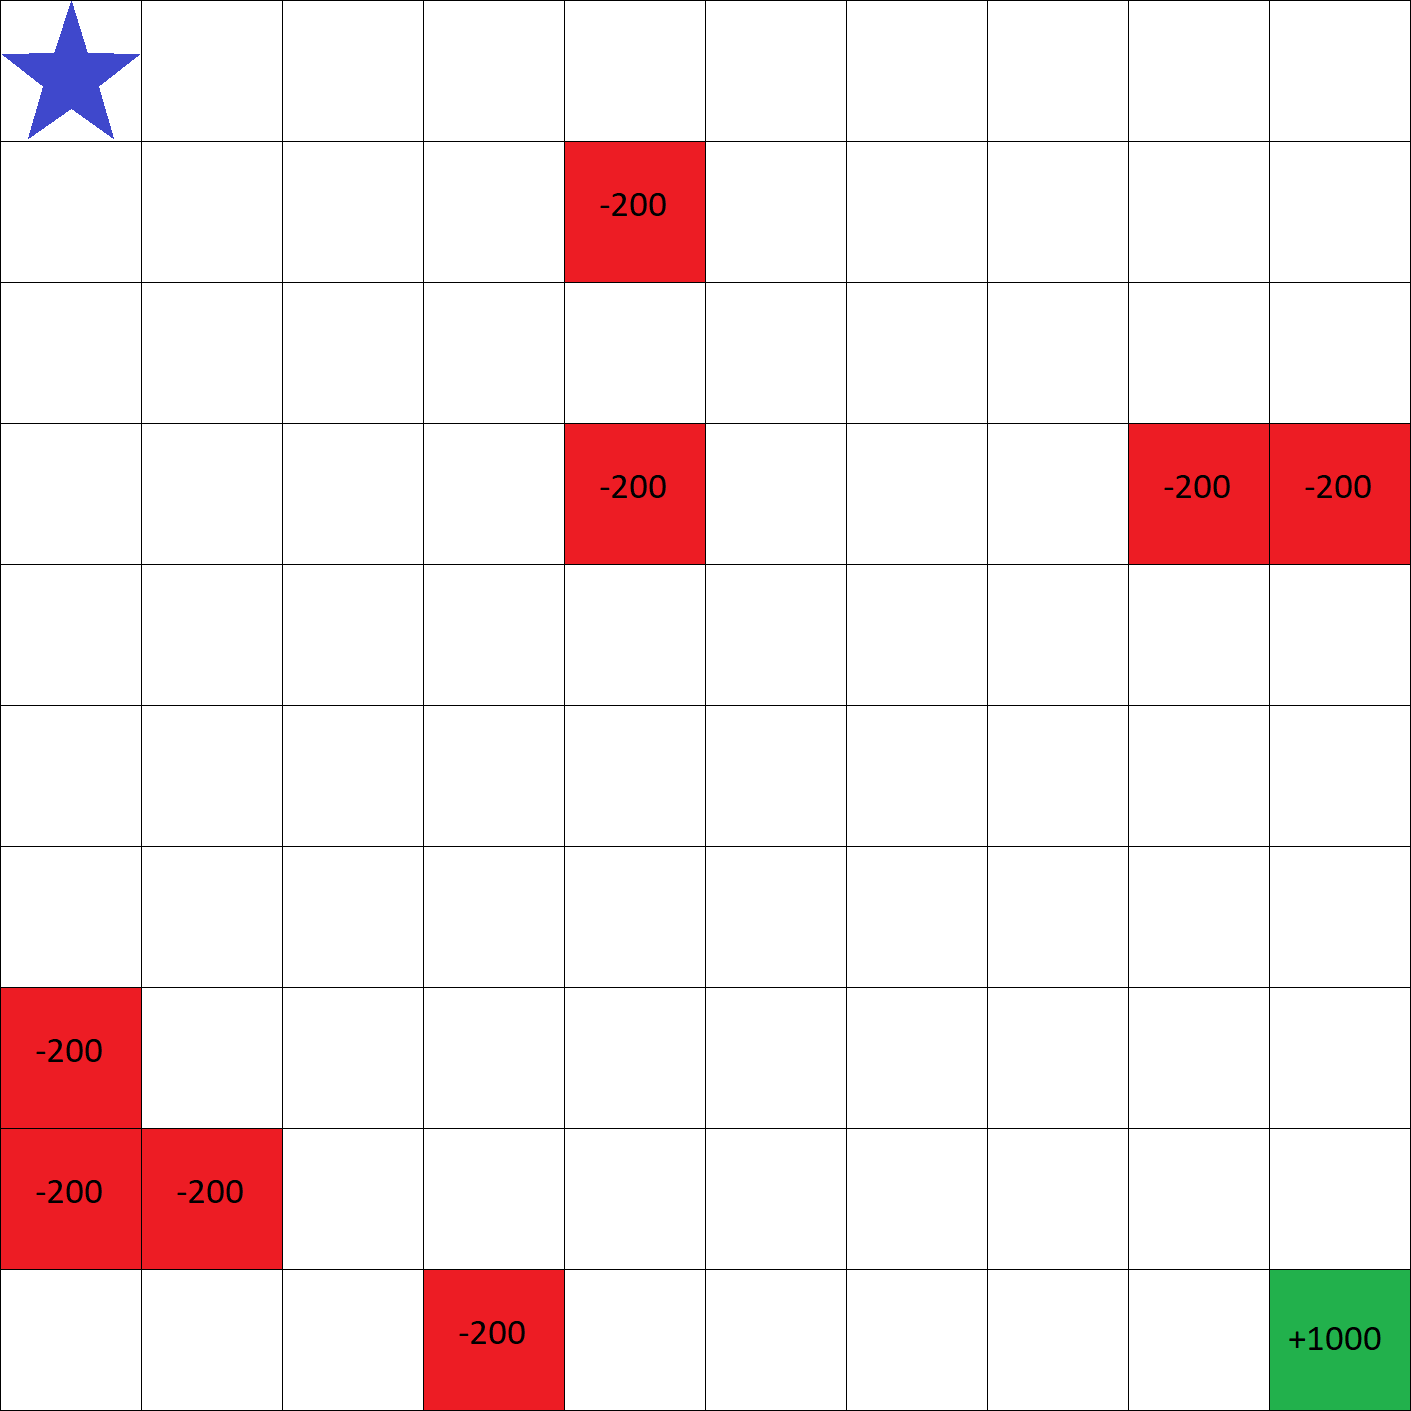
\includegraphics[scale=.2]{env_gridworld}
%  \caption{Mapa utilizado para os experimentos. A estrela azul indica a posição inicial do agente, o verde com +1000 representa o objetivo, e os vermelhos com -200 as armadilhas. Não há espaços inválidos.}
%  \label{fig:env_grid}
%\end{figure}

%\begin{figure}[h!]
%  \begin{minipage}[b]{.6\textwidth}
%  \centering
%  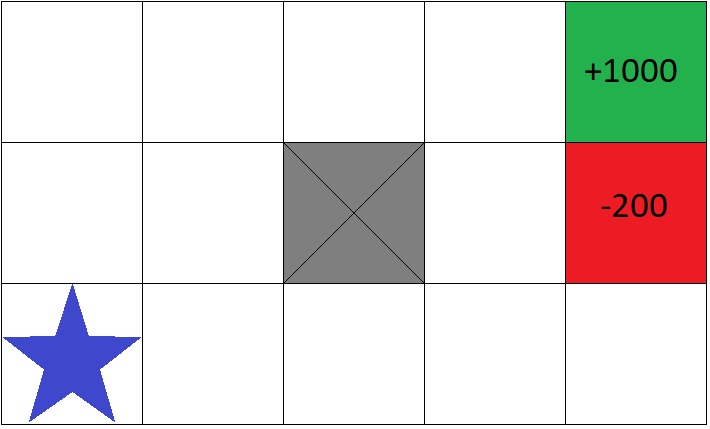
\includegraphics[scale=.35]{gridworld_example01}
%  %\caption{Exemplo de tela do jogo. O números no topo da tela são pontuação e quantidade de vidas respectivamente. A nave, no centro, está atirando. Asteroides espalhados pela tela.}
%  \end{minipage}
%  \hfill
%  \begin{minipage}[b]{.35\textwidth}
%  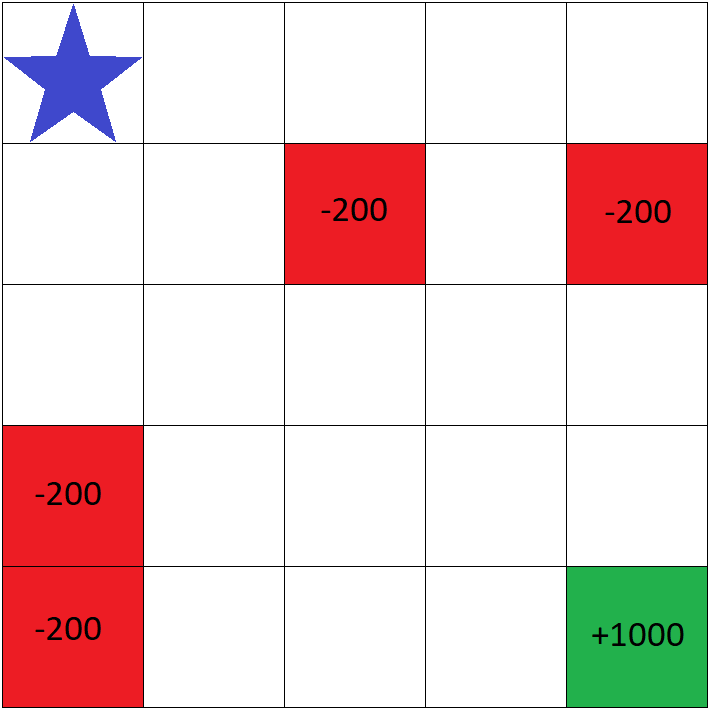
\includegraphics[scale=.2105]{gridworld_example02}
%  %\caption{Exemplo de tela do jogo. A nave acaba de destruir um asteroide de menor tamanho e está recebendo uma recompensa de 100 pontos por isso. Asteroides podem ter diversas cores.}
%  \end{minipage}
%  \centering
%  \caption{Exemplos de mapas de \textit{Gridworld}. A estrela azul indica a posição inicial do agente, o espaço cinza com um $\times$ indica um espaço inválido, o verde com +1000 representa o objetivo e os vermelhos com -200 representam as armadilhas.}
%\end{figure}

%O número de estados deste tipo de ambiente é igual ao número de espaços válidos, uma vez que são definidos pela posição em que o agente se encontra.
%Como os treinamentos foram feitos em um mapa de tamanho 10x10 sem espaços inválidos, o ambiente possui 100 estados com 4 ações possíveis em cada um.

%\subsection{\textit{Pong}}
%\label{sec:pong}
%
%\textit{Pong} foi um dos primeiros jogos criados e o primeiro desenvolvido pela Atari, lançado em novembro de 1972.
%O jogo simula uma partida de tênis de mesa por meio de duas barras verticais, uma do lado esquerdo e uma do lado direito, e uma bola que se move pela tela.
%Cada jogador controla uma das barras movendo-a para cima e para baixo, rebatendo a bola para evitar que chegue ao fim da tela do próprio lado enquanto tenta fazê-la chegar ao fim da tela do lado do adversário.
%A principal diferença entre as versões do jogo é o número de pontos necessário para vencer, que é de 21 no caso da utilizada neste trabalho, do Atari 2600.
%A versão do \textit{Pong} utilizada neste trabalho é a do Atari 2600, emulada pelo emulador Stella~\cite{stella}, na qual vence o jogador que fizer 21 pontos primeiro.

%\begin{figure}[h!]
%  \begin{minipage}[b]{.5\textwidth}
%  \centering
%  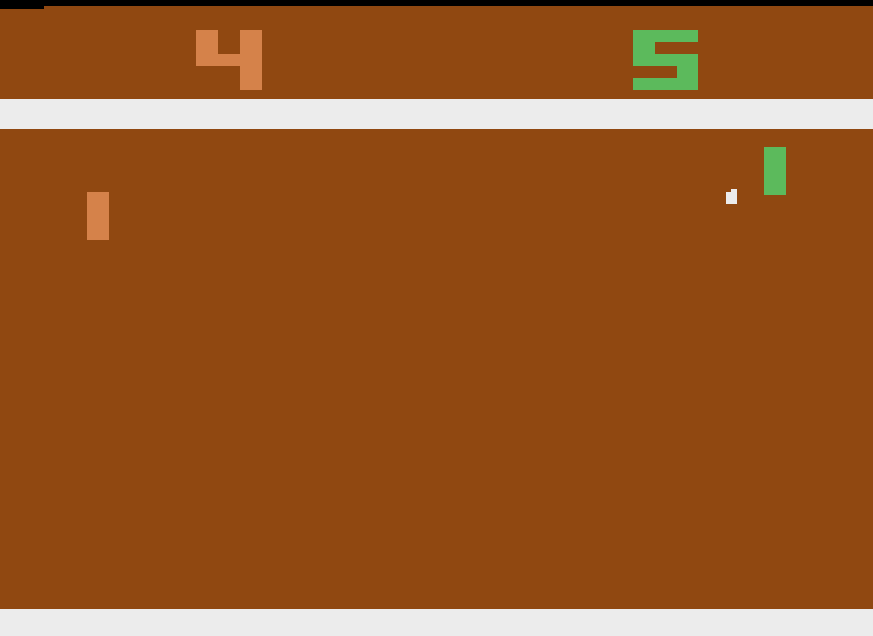
\includegraphics[scale=.25]{pong_example01}
%  %\caption{Exemplo de tela do jogo. O números no topo da tela são pontuação e quantidade de vidas respectivamente. A nave, no centro, está atirando. Asteroides espalhados pela tela.}
%  \end{minipage}
%  \hfill
%  \begin{minipage}[b]{.5\textwidth}
%  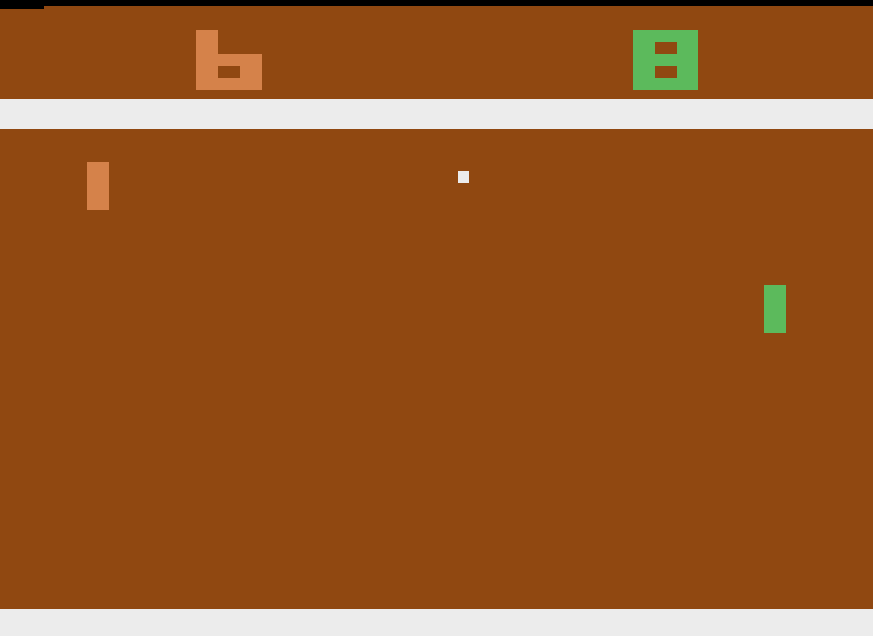
\includegraphics[scale=.25]{pong_example02}
%  %\caption{Exemplo de tela do jogo. A nave acaba de destruir um asteroide de menor tamanho e está recebendo uma recompensa de 100 pontos por isso. Asteroides podem ter diversas cores.}
%  \end{minipage}
%  \caption{Exemplos de tela do jogo no emulador de Atari 2600, Stella~\cite{stella}. Nestas imagens, o jogador controla a barra verde, do lado direito da tela, enquanto a IA criada pelos desenvolvedores do jogo controla a barra laranja, do lado esquerdo da tela. O ponto branco entre elas é a bola, as barras brancas horizontais que estendem desde o lado equerdo até o lado direito da tela representam os limites superior e inferior do campo, e os números no topo indicam a pontuação de cada jogador.}
%\end{figure}

%Os estados são definidos pela tela do jogo, que é uma matriz de 210x160 pixels, cada um sendo representado por 3 canais cujos valores variam de 0 a 255 para determinar a cor do pixel dentre 128 cores disponíveis, o que significa que muitas das combinações resultam nas mesmas cores.
%Esses números se traduzem em 33600 pixels e, portanto, $128^{33600}$ estados possíveis.
%Mesmo que apenas uma parcela deles sejam utilizados, é evidente que há muitos estados a mais que o \textit{Gridworld}.

%Uma vez que o agente deverá aprender observando a tela, o número de estados é proporcional ao número de pixels e quais cores podem assumir.

%\subsection{\textit{Asteroids}}
%\label{sec:asteroids}
%
%\textit{Asteroids} é um jogo de fliperama
%%do gênero \textit{top down shooter} (jogo eletrônico de tiro visto de cima)
%lançado em novembro de 1979 pela
%%então desenvolvedora de jogos eletrônicos Atari Inc, atualmente conhecida como
%Atari.
%O jogador controla uma nave espacial em um campo de asteroides e seu objetivo é destruir todos os presentes na tela enquanto desvia deles.
%Quando um asteroide é destruído, outros menores aparecem no lugar.
%O jogador possui cinco ações disponíveis: mover-se para frente, girar a nave no sentido horário, girar a nave no sentido anti-horário, mover-se no hiperespaço, e atirar para frente.
%Mover-se para frente e girar são as principais formas de movimento no jogo, enquanto atirar é a de destruir asteroides e ganhar pontos.
%Mover-se no hiperespaço consiste em fazer a nave desaparecer por alguns instantes e reaparecer em um local aleatório da tela.
%As principais diferenças entre as iterações de \textit{Asteroids} incluem a presença de naves espaciais inimigas que atiram contra o jogador, formatos e tamanhos diferentes dos asteroides, e direção em que se movem.
%A versão de \textit{Asteroids} utilizada neste trabalho é a do Atari 2600, com 4 vidas inicialmente, sem naves espaciais inimigas e três tamanhos distintos de asteroides, com o maior gerando uma recompensa de 20 pontos ao ser destruído, o médio gerando 50, e o menor 100, todos com movimento principalmente vertical.
%
%\begin{figure}[h!]
%  \begin{minipage}[b]{.5\textwidth}
%  \centering
%  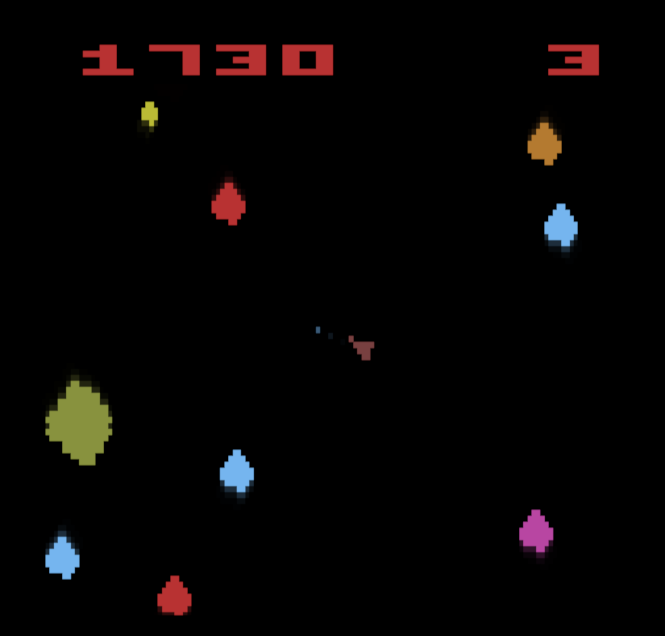
\includegraphics[scale=1.41]{asteroids_example01}
%  %\caption{Exemplo de tela do jogo. O números no topo da tela são pontuação e quantidade de vidas respectivamente. A nave, no centro, está atirando. Asteroides espalhados pela tela.}
%  \end{minipage}
%  \hfill
%  \begin{minipage}[b]{.5\textwidth}
%  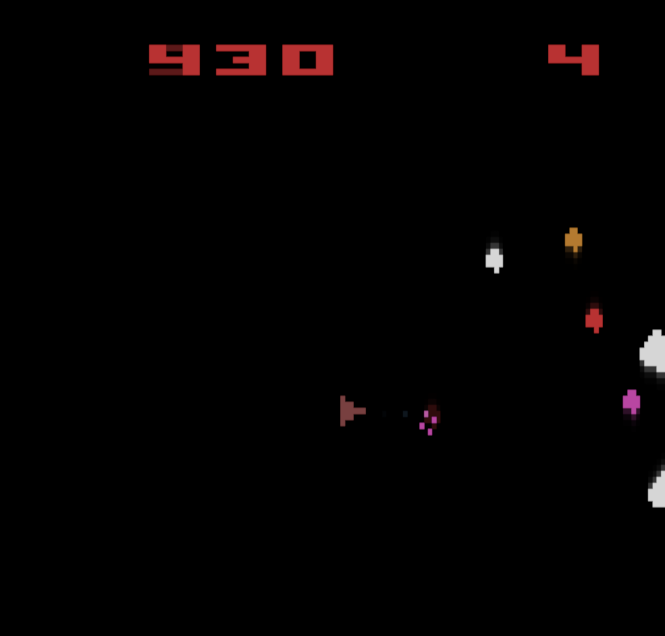
\includegraphics[scale=1.41]{asteroids_example02}
%  %\caption{Exemplo de tela do jogo. A nave acaba de destruir um asteroide de menor tamanho e está recebendo uma recompensa de 100 pontos por isso. Asteroides podem ter diversas cores.}
%  \end{minipage}
%  \caption{Exemplos de tela do jogo no emulador de Atari 2600, Stella. O número no canto superior esquerdo é a pontuação e o no canto superior direito é a quantidade de vidas restante que o jogador tem. A nave é o triângulo no meio da tela, o ponto azul próximo dela na imagem da esquerda é um tiro e o restante é asteroide. Na imagem da direita, os quatro pequenos pontos rosas próximos da nave são um asteroide que acaba de ser destruído.}
%\end{figure}
%
%Assim como no \textit{Pong}, os estados são compostos por uma matriz de 210x160 pixels, cada um sendo representado por 3 canais que determinam a cor, o que significa que possui a mesma quantidade de estados, com apenas uma parcela sendo utilizada.
%
%%Assim como no \textit{Pong}, o número de estados é proporcional ao número de pixels na tela e as cores que podem ter.

%------------------------%

\subsection{Gym \& Gym-Retro}
\label{sec:gymretro}

Gym é uma plataforma para pesquisa de aprendizado por reforço desenvolvida e mantida pela empresa de pesquisas em inteligência artificial OpenAI.
Esta ferramenta auxilia na emulação de diversos ambientes diferentes, incluindo alguns jogos de Atari 2600, e ambientes 3D.

Gym-Retro é uma variante da Gym com ênfase em jogos eletrônicos antigos, como dos consoles Sega Genesis, Nintendo Entertainment System e Atari 2600.
Para qualquer jogo que o usuário deseje emular, é necessário que ele tenha a ROM \footnote{\textit{Read Only Memory}: Memória Somente de Leitura, no contexto de emulação de jogos eletrônicos, é um tipo de arquivo copiado do chip de memória somente de leitura de cartuchos de jogos digitais. Eles são utilizados por emuladores para serem jogados em plataformas diferentes.} do jogo.

Foram utilizados dois ambientes do Gym neste trabalho, o \textit{Frozen Lake} e o \textit{Pong}, e um do Gym-Retro, o \textit{Asteroids}.
O \textit{Frozen Lake} é quase igual ao \textit{Gridworld}, com a diferença de haver aleatoriedade nos movimentos, ou seja, é possível o agente escolher mover-se para um lado, mas deslocar-se para outro, e haver apenas duas configurações de mapa pré-existentes: um de quatro linhas por quatro colunas (4x4) e um de oito linhas por oito colunas de espaços (8x8).
Para que ele pudesse ser utilizado como um \textit{Gridworld}, a aleatoriedade dos movimentos foi removida e mapas personalizados foram criados.
O ambiente do \textit{Pong} e do \textit{Asteroids} foram utilizados conforme disponibilizados pelas respectivas ferramentas, que utilizam o emulador de Atari 2600, Stella~\cite{stella}.
Os três ambientes são descritos com mais detalhes na seção \hyperref[sec:envs]{Ambientes} do capítulo 3, \hyperref[cap:implementacao]{Implementação}.
%O \textit{Pong} utilizado foi o disponibilizado pela ferramenta.
%Utilizou-se o \textit{Frozen Lake}, removendo a aleatoriedade dos movimentos e criando um mapa personalizado do tamanho desejado, e o \textit{Pong} do Gym neste trabalho.

%Gym-Retro é uma plataforma para pesquisa de aprendizado por reforços e generalização em jogos desenvolvida e mantida pela empresa de pesquisas em inteligência artificial OpenAI.
%Essa ferramenta auxilia na emulação de diversos consoles de jogos eletrônicos, como Sega Genesis, Nintendo Entertainment System (NES) e Atari 2600.
%Utilizou-se o \textit{Asteroids} do Gym-Retro neste trabalho.

%O principal motivo de estas ferramentas terem sido escolhidas é por permitirem emular o \textit{Pong} e o \textit{Asteroids}, além de possuir um ambiente semelhante ao \textit{Gridworld}.
%------------------------%
\subsection{TensorFlow}
\label{sec:tensorflow}

TensorFlow é um arcabouço de código aberto para computações numéricas de alta performance sobre tensores, desenvolvido e mantido pela Google.
Seu núcleo de computação numérica flexível permite o uso da biblioteca em diversos campos científicos, oferecendo, em particular, grande suporte a aprendizado de máquina e aprendizado profundo.
Esta ferramenta foi escolhida por oferecer uma API em Python estável, ter grande suporte, comunidade ativa, e ser de código aberto, sendo uma escolha sólida para a construção da rede neural.

%------------------------%

%\section{Proposta}
%\label{sec:proposta}
%
%A proposta deste trabalho é fazer um estudo de caso da técnica \textit{deep Q-learning} em três ambientes digitais diferentes e ver o grau de sucesso obtido em cada um, utilizando como entrada apenas a tela do jogo (considerando o mapa do \textit{Gridworld} com o agente inserido como uma tela).
%Gym e Gym-Retro servirão de interface enquanto o Stella emulará o jogo.
%As técnicas de aprendizado de máquina utilizadas serão \textbf{aprendizado por reforço} e \textbf{rede neural convolucional}, em particular o \textbf{\textit{deep Q-learning}}, que é a junção dessas duas.

%A proposta do trabalho é criar uma arquitetura para que uma inteligência artificial seja capaz de aprender a jogar \textit{Asteroids} do Atari 2600 tendo como entrada de dados apenas a tela do jogo, representada por uma matriz de pixels de 210x160 e 3 canais de cores.
%O emulador Stella e o Gym-Retro serão utilizados para emular o jogo e servir de interface com o jogo respectivamente.
